From the given information, the hicker's position vector is 
\begin{align}
\vec {A} = \myvec{0\\490}
\end{align}
the acceleration of the stone is 
\begin{align}
\vec a = \myvec{0\\-9.8}
\end{align}
and the initial velocity of the stone is 
\begin{align}
\vec {v}_A = \myvec{1.5\\0}
\end{align}
If $\vec{B}$ be the final position of the stone, 
\begin{align}
\label{eq:3.8.4_vb}
\vec {v}_B &=  \vec {v}_A  + \vec{a} t
\\
\vec{B} &= \vec{A}+\vec {v}_A t + \frac{1}{2}\vec {a} t^2
\\
\implies \vec{B}= \myvec {x\\0}  &= \myvec{0\\490} + \myvec{1.5\\0}t +\frac{1}{2}\myvec{0\\-9.8} t^2
\label{eq:3.8.4_b}
\end{align}
$\because$ the stone finally comes to rest.  Thus, 
\begin{align}
490 &= \frac{1}{2} 9.8t^2
\\
\implies t &= 10
\end{align}
Substituting in \eqref{eq:3.8.4_vb}, 
\begin{align}
\vec v_B &= \myvec{1.5\\0} + \myvec{0\\9.8}10 
\\
&= \myvec{1.5\\98}
\end{align}
The final speed is given by $\norm{\vec{v}_B}$.
The motion of the stone is plotted in Fig. \ref{fig:3.8.3_motion} using \eqref{eq:3.8.4_b} by varying $t$ through the following code.
%
\begin{lstlisting}
solutions/4/codes/line/motion/motion.py
\end{lstlisting}
\begin{figure}[!ht] \centering 
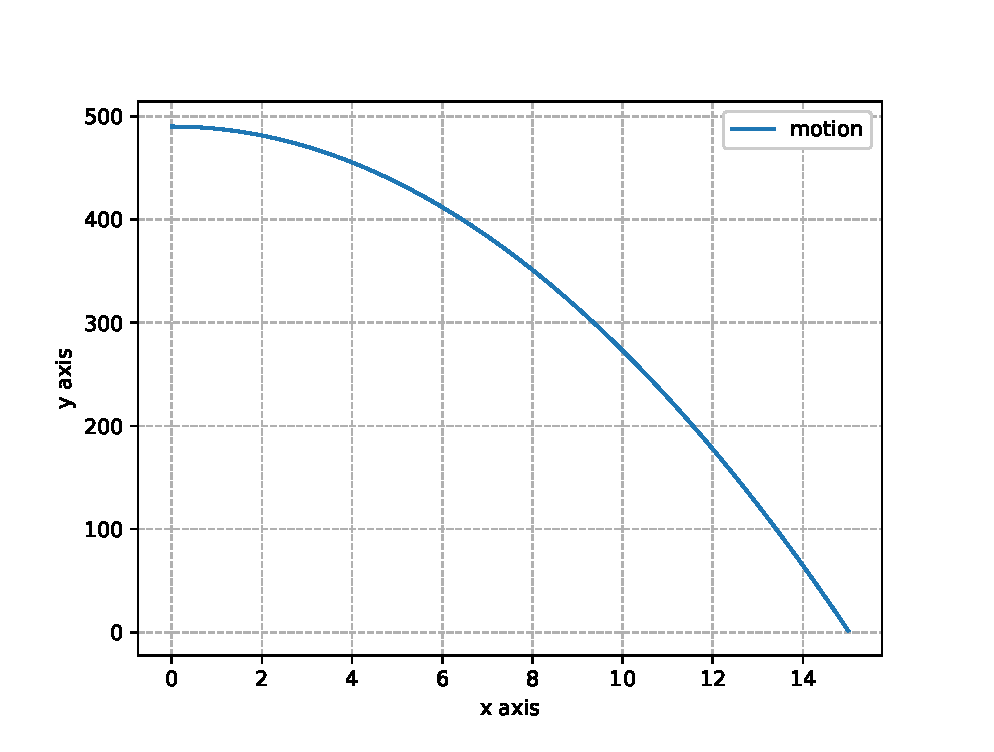
\includegraphics[width=\columnwidth]{./solutions/4/figures/line/motion/motion.eps} \caption{} 
\label{fig:3.8.3_motion} \end{figure}

